\documentclass{beamer}
\usepackage[ruled,vlined,boxed]{algorithm2e}
\usepackage{adjustbox}

\setbeamertemplate{bibliography item}{\insertbiblabel}

\usetheme{Madrid}



\title{Software Component Identification and Composition}
\institute[MNNIT]{
	
\includegraphics[height = 1.5cm]{logo.jpg}\\
	\normalsize{Computer Science \& Engineering Department}\\
	Motilal Nehru National Institute of Technology\\
	Allahabad, Prayagraj\\
}
\author[Anshuman Sekhar Dash]{
	\normalsize{Presented By}\\
	\Large{Anshuman Sekhar Dash}\\
	\normalsize{
		M.Tech. 3\textsuperscript{rd} Sem\\
		Information Security\\
		Reg No: 2020IS04}
}
\begin{document}
\begin{frame}[plain]
    \maketitle
\end{frame}
\begin{frame}{Outline}
	\tableofcontents
\end{frame}
\section{Introduction}
\begin{frame}[allowframebreaks]{Introduction}
	\begin{itemize}
		\item From the last 10 years use of computer software has entered into every part of economy which has in turn generated new demand from the software industry to develop reliable and cost effective software quickly and efficiently.
		\item Modern software systems are becoming more and more large scale which further increases the development cost , decreases the productivity and increases the cost of maintenance.
		\item A software system need not be developed all the way from scratch and instead the software system can be developed by piecing together small pieces of software from previously developed software system and assembling them to make a final product.
		
		\item In the context of CBSE a component will be defined as a unit of composition with contractually specified interfaces and explicit context	dependencies only.
		\item A software component can be deployed independently and is subject to composition by third parties.
		
		\item The primary role of CBSE is to direct making of software system as stitching of parts or components , development of the individual components as reusable entities and maintenance of the system developed with timely replacement of components\cite{9497978}.
	\end{itemize}
\end{frame}
\begin{frame}
	\begin{figure}
		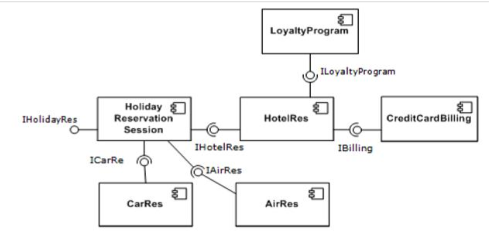
\includegraphics[scale=0.5]{softwareComponentExample.png}
		\caption{Software Components Example}
	\end{figure}
\end{frame}
\section{Software Component Problem}
\begin{frame}{Software Component Identification Problem}
	\begin{itemize}
		\item Component identification during the software design phase is a process in which the functionalities of a given system are partitioned into non intersecting logical components to provide the starting point for designing software architecture \cite{survey}\cite{componentDef}.
		\item It is a complex problem and depends on
		different parameters with variable values and limiting conditions.
		\item This component identification problem belongs to Non-polynomial time problem which can only be solved by
		exhaustive search of all the different possibilities\cite{2}.
	\end{itemize}
\end{frame}
\begin{frame}{Software Composition Problem}
	\begin{itemize}
		\item Effective reuse of software components not only depends on identification of software components but also the ways to merge the components.
		\item The other problem in CBSE is that
		of Component composition.
		\item Presently object oriented programming languages provide ad-hoc mechanisms for composing software using components.
		\item By providing a proper semantic
		foundation definition we will be able to cleanly integrate all the requirements of the software
		system into one system\cite{softwareComposition}\cite{dynamicComp}.
	\end{itemize}
\end{frame}
\section{Previous Approaches}
\begin{frame}
	\begin{columns}
		\begin{column}{0.5\textwidth}
			\begin{table}
				\caption{Artefacts used }
				\begin{adjustbox}{width=\columnwidth,center}
					\begin{tabular}{|c c |} 
						\hline
						Artefact & References  \\ 
						\hline\hline
						Static/dynamic Call graphs & \cite{graphPartion}  \\ 
						\hline
						Use Cases & \cite{neural}\cite{genetic}\cite{CRUD} \\
						\hline
						Source Code  & \cite{graphPartion} \\
						\hline
						Sequence Diagram & \cite{CRUD}\cite{2}  \\
						\hline
						Relationship between classes & \cite{genetic}  \\ [1ex] 
						\hline
						Business Model Documents & \cite{graphPartion}\cite{FCA}  \\ [1ex]
						\hline
						Class Diagrams & \cite{genetic}\cite{CRUD}\cite{ClusteringClass}  \\ [1ex]
						\hline
						Requirements Definition & \cite{highCohesionLowCoupling}  \\ [1ex]
						\hline
						Collaboration Diagram & \cite{FCA}  \\ [1ex]
						\hline
					\end{tabular}
				\end{adjustbox}
			\end{table}
		\end{column}
	\begin{column}{0.5\textwidth}
		\begin{table}
			\caption{Component Identification Techniques}
				\begin{adjustbox}{width=\columnwidth,center}
				\begin{tabular}{|c c |} 
					\hline
					Methods & References  \\
					\hline\hline
					High cohesion and Low coupling & \cite{highCohesionLowCoupling}  \\ 
					\hline
					Use Case & \cite{useCase} \\
					\hline
					Fuzzy based analysis & \cite{fuzzy}  \\ [0.5ex]
					\hline
					Artificial Neural Network  & \cite{neural} \\
					\hline
					Genetic Algorithm & \cite{genetic}  \\
					\hline
					Particle Swarm Optimization & \cite{pso}\cite{pso1}  \\ [1ex] 
					\hline
					\textbf{Other Methods} &   \\
					\hline
					CRUD Based & \cite{CRUD}  \\ 
					\hline
					Graph Partitioning & \cite{graphPartion}  \\ 
					\hline
				\end{tabular}
			\end{adjustbox}
		\end{table}
	\end{column}
	\end{columns}
\end{frame}
\begin{frame}{Clustering Approaches}
\begin{enumerate}
	\item \textbf{High cohesion and Low Coupling:-}\cite{highCohesionLowCoupling} used high cohesion and low coupling metric to cluster classes into logical components.Key classes were selected by an expert.Other classes were assigned any one among these classes based on level of dependency.It was very much dependent on the expert since key classes were required to be chosen
	\item \textbf{Use Case:-} Use case,object models and collaboration diagrams were used to identify components.Clustering was performed on functional dependencies of use cases.In \cite{KMeans}\cite{agglomerative} all the different types of clustering algorithms present were used and compared.It required weighting by an expert\cite{clusteringAna}.
\end{enumerate}
\end{frame}
\begin{frame}[allowframebreaks]{Artificial Neural Network}
	\begin{itemize}
		\item \cite{neural} used designing phase use case diagrams and components was generated using neural network that was self organized.
		\item The criterion for neural network was cohesion and coupling.
		
		\item The number of neurons required initially is static and any change in use case the process needs to be repeated from starting.
	\end{itemize}
	 
\end{frame}
\begin{frame}{Genetic Algorithm}
	\begin{itemize}
		\item In genetic algorithm both the cohesion and coupling between two components is combined into a single objective function.
		\item This metric is then used to reject components whose fitness value is low\cite{genetic}.
		\item Genetic algorithm generated good results in small scale systems but failed to reciprocate good results in large scale system because in large scale systems probability of getting a good initial population is very low\cite{evolution}.
	\end{itemize}
		
		\end{frame}
	\begin{frame}{Particle Swarm Optimization}
		\begin{itemize}
			\item PSO is a computational and artificial intelligence technique\cite{pso1}.
			\item The important factor of PSO which distinguishes it from other is its fast convergence in compression with other algorithms of global optimization.
			\item Feature vector is used to represent a class.
			\item Shortcomings of this approach is that it can only be used with object oriented systems.
		\end{itemize}
		

\end{frame}
\begin{frame}{Formal Concept Analysis}
	\begin{itemize}
		\item FCA is a framework which uses mathematics that is used to
		explain and analyse data and their relationships\cite{FCA1}.
		\item \cite{FCA} uses a framework based on FCA that divides class diagram into logical components which is like that of clustering techniques.Adding on this paper \cite{FCA} used a new method that was based on fuzzy FCA.Dispersion and distance concept was used to calculate cohesion and coupling metrics.
		\item Fuzzy clustering  is useful when the boundaries between clusters are not well separated.
		\item Disadvantage of this method was that the threshold for dispersion and distance was set manually and it impacted heavily on the result, depends on the number of clusters and is susceptible to outliers in the components data.
	\end{itemize}
\end{frame}
\begin{frame}{Other Methods}
	\begin{enumerate}
		\item \textbf{Graph Partitioning:-}In paper \cite{graphPartion} object models was related with vertices and edges of graph.
		In graph partitioning technique the business model or the domain model is mapped into a weighted graph by an expert.This weighted graph is then used to apply graph segmentation technique .weights are manually assigned by experts.The graph is divided using heuristic from graph theories.The one disadvantage of this method is that it depends a lot on the weights given by the expert.The paper didn't justify the conclusion.
		\item \textbf{CRUD Based:-}The 4 relationship used in this method is Create, Read , Write ,Update and Delete with their priority set as $C > D > U > R$ and these relationship are used to give a semantic relationship.This relationship is then transformed into a matrix .\cite{CRUD} Used business events as inputs.
	\end{enumerate}
\end{frame}
\section{Formal Method Approach}
\begin{frame}{Constructing Software Library using formal Methods}
	We selected \cite{formal} and \cite{survey} as the base paper for our research work.\cite{formal} used formal language predicate logic to specify software components which can be used for both object oriented and function based systems.Since it only requires the source code to specify software components no domain level elements are required from the software system.\\
	Steps used in identification of software components using formal methods:-
	\begin{enumerate}
		\item Formal Specification of Software Components
		\item Generating Lower Level Hierarchy
		\item Measuring Similarity 
		\item Higher Level Hierarchy using Clustering
	\end{enumerate}
\end{frame}
\begin{frame}{Formal Specification of Software components}
	\begin{columns}
		\begin{column}{0.5\textwidth}
	\begin{itemize}
		\item Interface represents syntactic specification of the method.
		\item Type declarations represents the type of input output and local variables used.
		\item Precondition describes the condition of the variables before the method is called.
		\item Post condition describes the condition of the variables after the method is called.
	\end{itemize}
\end{column}
\begin{column}{0.5\textwidth}
	\begin{figure}
		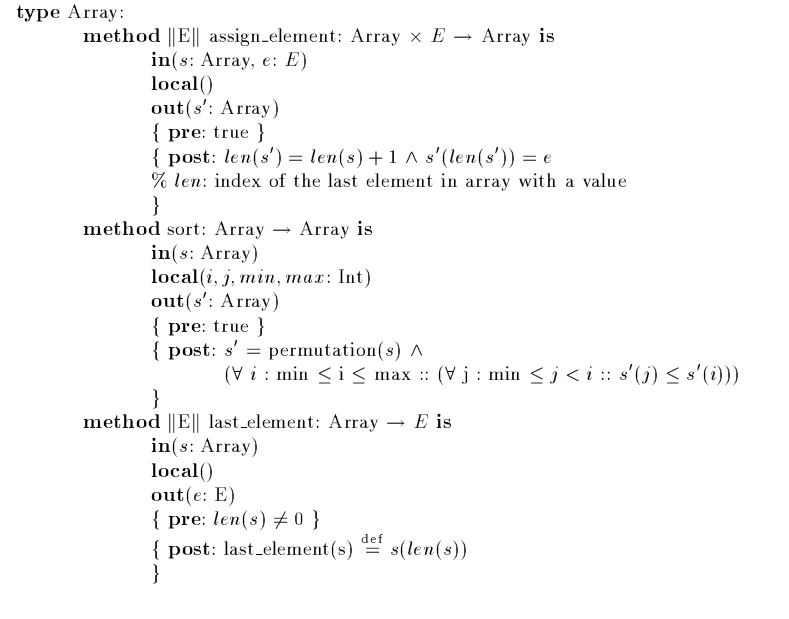
\includegraphics[scale=0.2]{example_formal.png}
		\caption{Example of predicate logic specification of component\cite{formal}}
		
	\end{figure}
\end{column}
	\end{columns}
\end{frame}
\begin{frame}[allowframebreaks]{Generating Lower Level Hierarchy}
	\begin{itemize}
		\item The lower level hierarchy will generate fine-grained components on which logical reasoning can be done on the basis of specifications.
		\item The subsumption relationship between 2 components will be used to classify and group together components which can be reused.
		\item A component is said to subsume another component when the first component is more general than the second.
		\item This abstract data type can be implemented on classes as class can also be termed as an abstract data type.
	\end{itemize}
\begin{algorithm}[H]
	\caption{Pair Wise Algorithm}
	\KwIn{The set of components from subsumption test algorithm $S=\{Cmp_1,Cmp_2,...,Cmp_n\}$}
	\KwOut{Hierarchy of components by applying generality principle}
	\While{$S\neq\{\}$}
	{
		choose some $Cmp_i \mathcal{E}  S $;\\
		$S \leftarrow S\div Cmp_i$;\\
		$set \leftarrow S$;\\
		\While{$set \neq \{\}$}
		{
			choose some $Cmp_j \mathcal{E}  S $;\\
			$S \leftarrow S\div Cmp_j$;\\
			\If{$C_i \sqsupseteq C_j$}
			{$C_i$ is set as parent of $C_j$ }
			\ElseIf
			{$C_j \sqsupseteq C_i$}
			{$C_j$ is set as parent of $C_i$}
		}
		
	}
\end{algorithm}
\end{frame}
\begin{frame}{Measuring Similarity}
\begin{itemize}
	\item Similarity of 2 components is represented as \(S(x,y)\).
	\item Example \(X=(C_1 \wedge C_2)\vee(C_2 \wedge C_3)\ and \ Y=(C_3)\vee(C_2 \wedge C_3)\)
	\item In the solution a component is represented in disjunctive normal form consisting of conjuncts. Each conjunct is to be associated
	with an equivalence class.
	\item For every component a matrix will be constructed whose dimensions are \(m \times (T+1)\) where m is the number of conjunction and T is the number of equivalence classes.
	\item 
		\(X(i,0) = u_i\;  0 \leqq i \leqq m \leqq 1\;
		and 
		X(i,j) = l\;  x_i\;has\;l\;terms\;in\;eq\;class\;j
		\)
	\item 	\(
	for\ all\ i,j\ if\ X(i,0)=Y(j,0)
	)\
	\)
	\\
	\(
	then\ s^{'} (i,j)=\frac{\sum_{t=1}^{T}2*min(X(i,t),Y(j,t))}{(X(i,t)+Y(j,t)}\)
	\\
	\(else\ s^{'}(i,j)=0
	\)
	\item 	\(s(X,Y)\)=$\frac{\sum_{i=1}^{m}\sum_{j=1}^{n}s^{'}(i,j)}{N}$
\end{itemize}
\end{frame}
\begin{frame}{Higher Level Hierarchy Using Clustering}
	\begin{itemize}
		\item In divisive algorithms the set X is further divided into a set of clusters using dissimilarity measure to form a finer partition.
		\item In agglomerative algorithms a group of finer partitions are merged together using
		similarity measures to form a courser partition.
		\item Each intermediate steps helps in generating a
		hierarchy of clusters.
		\item It provides an architectural understanding of the system.
		\item The agglomerative hierarchical clustering algorithms (AHCA) begin from a set of individual entities that are first allocated into small clusters which are then in turn allocated
		into larger clusters until reaching a final all inclusive clustering.
	\end{itemize}
\end{frame}
\begin{frame}{Agglomerative Clustering}
	\begin{algorithm}[H]
		\caption{Agglomerative Clustering}
		\KwIn{A Set of disjoint Lattices}
		\KwOut{Set of Clusters Unified into one}
		\begin{enumerate}
			\item each top element of the lattice is set a cluster with only single element
			\item search for a pair of clusters which have maximum similarity 
			\item merge the the top 2 most similar clusters into a new cluster
			\item calculate new similarity scores for the clusters left
			\item proceed until only one cluster is left
		\end{enumerate}
	\end{algorithm}
\end{frame}
\begin{frame}{Final Result}
	\begin{columns}
		\begin{column}{0.5\textwidth}

			\begin{figure}
				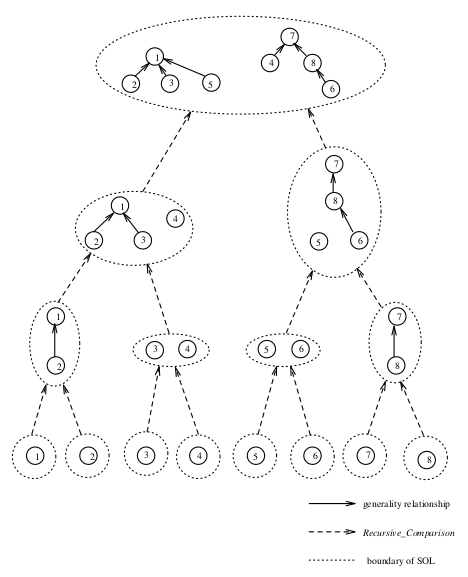
\includegraphics[scale=0.3]{lowerLevelHierarchy.png}
				\caption{Lower Level Hierarchy Building using recursive comparison\cite{formal}}
				
			\end{figure}

		\end{column}
		\begin{column}{0.5\textwidth}

			\begin{figure}
					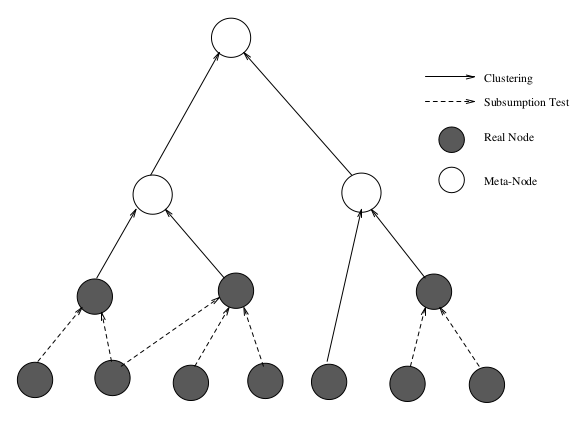
\includegraphics[scale=0.3]{finalHierarchy.png}
				\caption{Final resultant hierarchy of software components\cite{formal}}
				
			\end{figure}

		\end{column} 	
	\end{columns}
\end{frame}
\section{Conclusion}
\begin{frame}{Conclusion and Future Research}
	\begin{itemize}
		\item Most of the Approaches used Clustering for component identification but focussed mainly on top down approach
		\item Evolutionary techniques like particle swarm optimization and genetic algorithm gives better result but are limited to object oriented programming.
		\item Using formal methods to describe the source code and then using it to identify software components is the approach we will use for software component identification.
		\item Verification of software components using the idea from \cite{formalVerification}
		\item Next problem in CBSE is composing software using components where a providing a proper semantic definition will help in cleanly integrating all requirements of the software system into one system.
	\end{itemize}
\end{frame}
\section{References}
\begin{frame}[allowframebreaks]{References}
	\bibliographystyle{unsrt}
	\bibliography{ref}
\end{frame}
\begin{frame}
	\begin{center}
		Thank You!\\
		Any Questions?
	\end{center}
\end{frame}

\end{document}
